\section{Concepts}
\label{sec:concepts}
\subsection{Closed and Open Loop}
\label{subsec:concepts-closed-open-loop}
\begin{frame}{\insertsubsection}
	We distinguish between two different controllers
	\begin{itemize}
		\item Open Loop Controller
		\item Closed Loop Controller
		\item[ ] $\rightarrow$ Closed loop control schemes are the biologically more interesting ones.
	\end{itemize}
\end{frame}
%
%
\begin{frame}{\insertsubsection}
\begin{figure}
	\begin{tikzpicture}
		% Draw nodes
		\node [block] (controller) {Controller};
		\coordinate [left of=controller, node distance=3cm] (init);
		\node [block, right of=controller, node distance=5cm] (system) {System};
		\coordinate [right of=system, node distance=3cm] (end);
		% Draw lines connecting (arrows)
		\path [line] (init) -- node [midway, above] {Input} (controller);
		\path [line] (controller) -- node [midway, above] {Control Signal} (system);
		\path [line] (system) -- node [midway, above] {Output} (end);
	\end{tikzpicture}
	\caption{Open Loop Control System}
\end{figure}
\end{frame}
%
%
\begin{frame}{\insertsubsection}
\begin{figure}
	\begin{tikzpicture}
		% Draw nodes
		\node [block] (controller) {Controller};
		\node [block, right=3cm of controller] (system) {System};
		\node [block, below right=0.5cm and 0.5cm of controller] (measurement) {Measurement};
		% Helper coordinates
		\coordinate [left=2cm of controller] (init);
		\coordinate [right=2cm of system] (end);
		\coordinate [right=1cm of system] (measurepoint);
		\coordinate [below right=0.5cm and 5cm of controller] (rightcorner);
		\coordinate [below of=controller] (leftcorner);
		% Draw lines connecting (arrows)
		\path [line] (init) -- node [midway, above] {Input} (controller);
		\path [line] (controller) -- node [midway, above] {Control Signal} (system);
		\path [line] (system) -- node [midway, above] {Output} (end);
		% \path [line] (measurepoint) -- (rightcorner) -- (measurement);
		%\draw (measurepoint) to (rightcorner) to (measurement) to (leftcorner) to (controller);
		\path [line] (measurepoint) |- (measurement);
		\path [line] (measurement) -| (controller);
	\end{tikzpicture}
	\caption{Closed Loop Control System with Measurement and Feedback}
\end{figure}
\end{frame}
%
%
\subsection{Controller Types}
\label{subsec:concepts-controller-types}
\begin{frame}{\insertsubsection}
	\begin{figure}
		\centering
		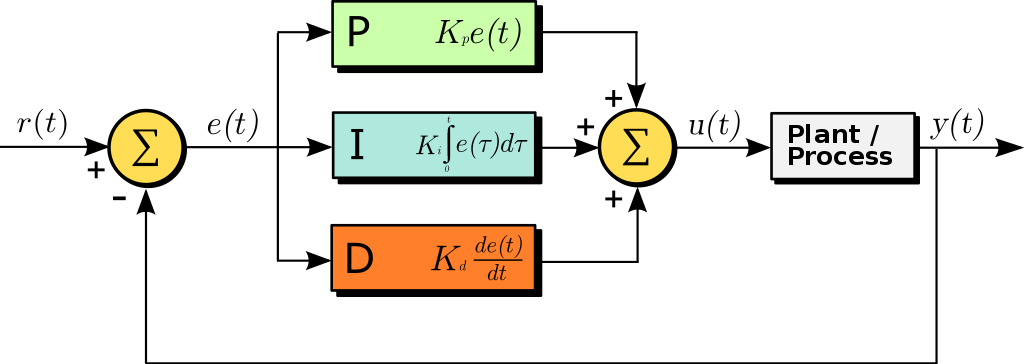
\includegraphics[width=\textwidth]{media/PID_en}
		\caption{Schematic Overview of a Controller~\cite{wikiPID2011}}
	\end{figure}
	Relevant values:\\
	$u(t)$ - Response of controller\\
	$e(t)$ - Difference of input signal and setpoint (target)
	\begin{equation}
		e(t) = r(t) - y(t)
	\end{equation}
\end{frame}
%
%
\subsubsection{Proportional (P) Controller}
\label{subsec:concepts-controller-types-p-controller}
\begin{frame}{\insertsubsubsection}
	$u(t)$ - Response of controller\\
	$e(t)$ - Difference of input signal and setpoint (target)\\\\
	We want to calculate response $u(t)$ from input $e(t)$.\\
	Use a proportional response
	\begin{equation}
		u(t) = K_P e(t)
	\end{equation}
\end{frame}
%
%
\subsubsection{Differential (D) Controller}
\label{subsec:concepts-controller-types-d-controller}
\begin{frame}{\insertsubsubsection}
	$u(t)$ - Response of controller\\
	$e(t)$ - Difference of input signal and setpoint (target)\\\\
	Differential response
	\begin{equation}
		u(t) = K_D \frac{\partial e}{\partial t}
	\end{equation}
	In discretized version
	\begin{equation}
		u(t_{i+1}) = K_D \frac{e(t_{i+1})- e(t_i)}{\Delta t}
	\end{equation}
\end{frame}
%
%
\subsubsection{Integral (I) Controller}
\label{subsec:concepts-controller-types}
\begin{frame}{\insertsubsubsection}
	$u(t)$ - Response of controller\\
	$e(t)$ - Difference of input signal and setpoint (target)\\\\
	Differential response
	\begin{equation}
		u(t) = K_I \int\limits^t_0 e(\tau)d\tau
	\end{equation}
	In discretized version
	\begin{equation}
		u(t_{n+1}) = K_I \sum\limits_{i=0}^n e(t_i)\Delta t
	\end{equation}
\end{frame}
%
%
\subsection{Combinations of Controller}
\label{subsec:concepts-combinations}
\begin{frame}{\insertsubsection}
	We can combine the previously introduced controllers.\\
	PD Controller
	\begin{equation}
		u(t) = K_P e(t) + K_D \frac{\partial e}{\partial t}
	\end{equation}
	PI Controller
	\begin{equation}
		u(t) = K_P e(t) + K_I \int\limits^t_0 e(\tau)d\tau
	\end{equation}
	PID Controller
	\begin{equation}
		u(t) = K_P e(t) + K_I \int\limits^t_0 e(\tau)d\tau + K_D \frac{\partial e}{\partial t}
	\end{equation}
	...
\end{frame}
%
%
\subsubsection{Controller Constants}
\label{subsec:concepts-controller-constant-discussion}
\begin{frame}{\insertsubsubsection}
	\begin{figure}
		\centering
		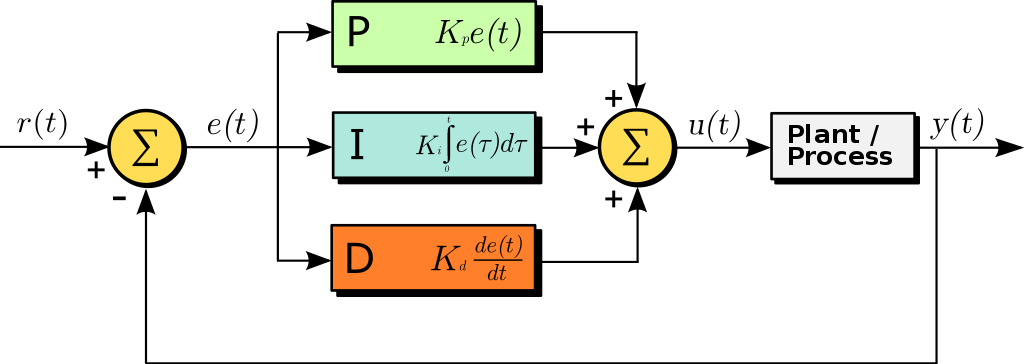
\includegraphics[width=\textwidth]{media/PID_en}
		\caption{Schematic Overview of a PID Controller~\cite{wikiPID2011}}
	\end{figure}
	\begin{align}
		e(t) &= r(t) - y(t)\\
		u(t) &= K_P e(t) + K_I \int\limits^t_0 e(\tau)d\tau + K_D \frac{\partial e}{\partial t}
	\end{align}
\end{frame}
%
%
\begin{frame}{\insertsubsubsection}
	What do the parameters $K_P, K_I, K_D$ do?
	\begin{equation}
		u(t) = K_P e(t) + K_I \int\limits^t_0 e(\tau)d\tau + K_D \frac{\partial e}{\partial t}
	\end{equation}
	Alternative representation
	\begin{equation}
		u(t) = K_P \left(e(t) + \frac{1}{T_I}\int\limits^t_0 e(\tau)d\tau + T_D\frac{\partial e}{\partial t}\right)
	\end{equation}
	What do $K_p,T_I,T_D$ do now?
\end{frame}
%
%
\begin{frame}{\insertsubsubsection}
	\begin{figure}
		\centering
		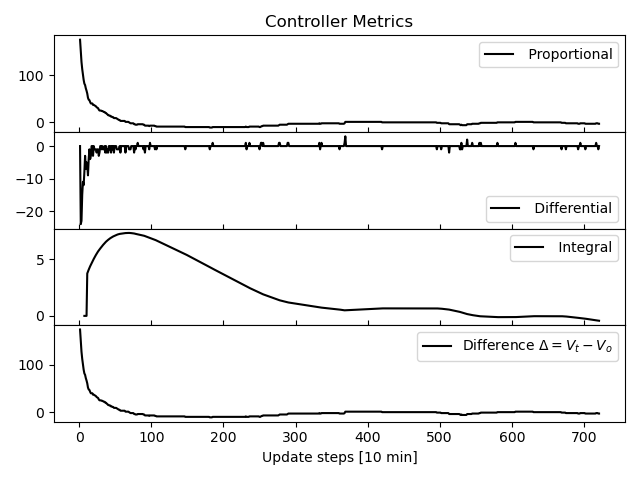
\includegraphics[width=0.8\textwidth]{media/UkrainianFlagControllerMetrics}
		\caption{Optimal Control for a given system.}
	\end{figure}
\end{frame}
%
%
\begin{frame}{\insertsubsubsection}
	\begin{figure}
		\centering
		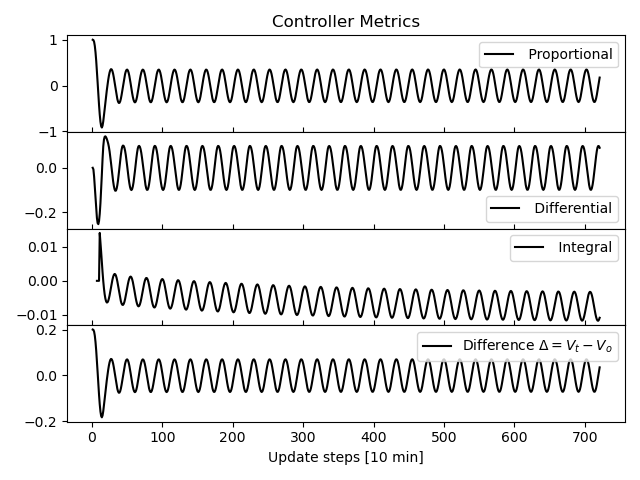
\includegraphics[width=0.8\textwidth]{media/TimeDelayOscillations}
		\caption{Oscillations can occur upon time-delays are.}
	\end{figure}
\end{frame}
%
%
\subsection{Optogenetic Control}
\label{subsec:concepts-optogenetic-control}
\begin{frame}{\insertsubsubsection}
	\begin{figure}
		\centering
		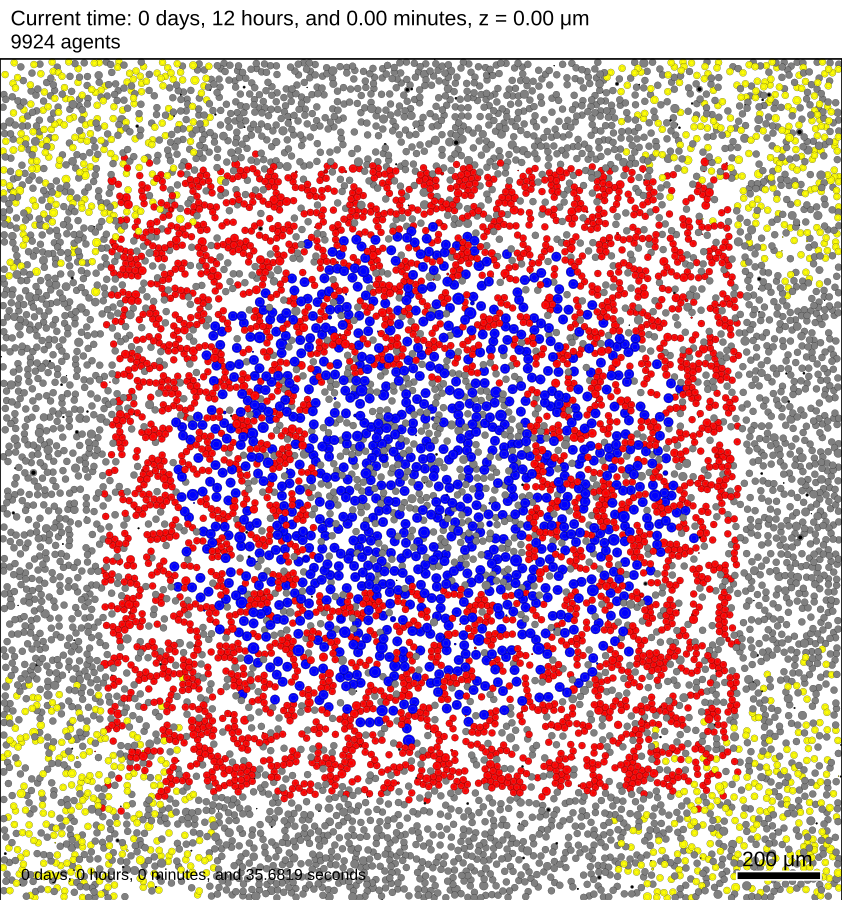
\includegraphics[width=0.6\textwidth]{media/SpatialDensityControl}
		\caption{Optogenetic controllers regulate cell densities in different spatial compartiments.}
	\end{figure}
\end{frame}